\begin{figure}[h]
    \centering
    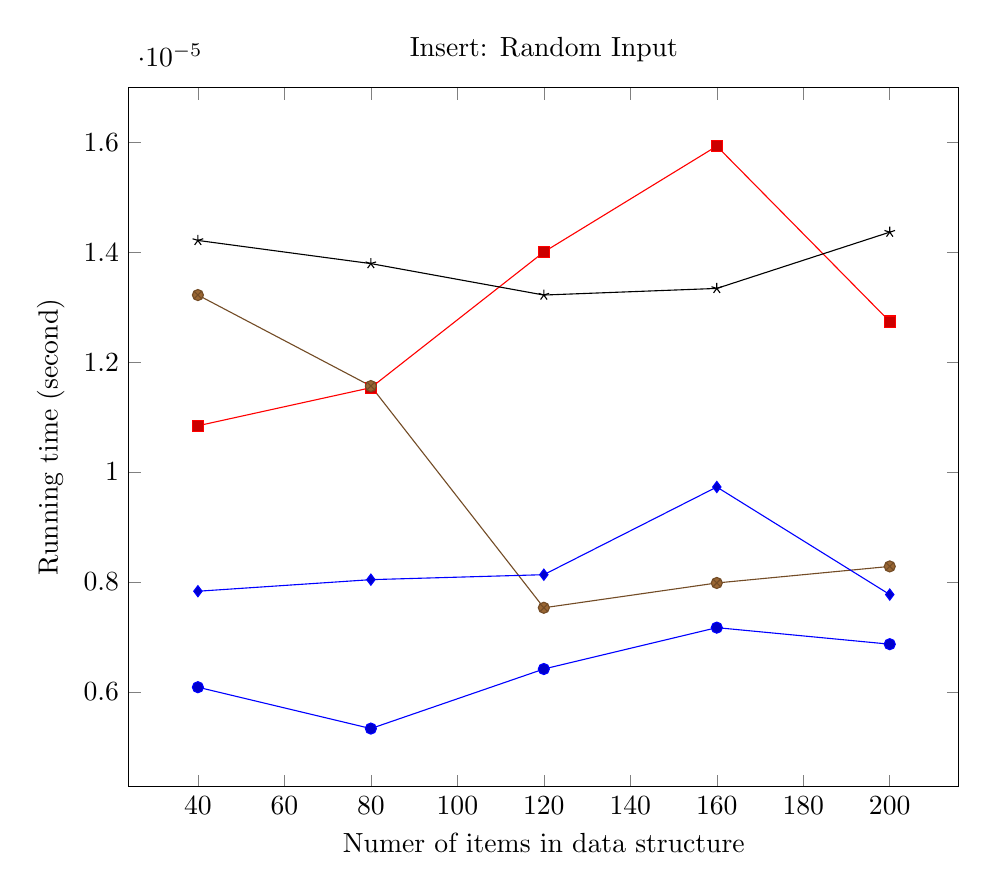
\begin{tikzpicture}
        \begin{axis}[
            xlabel={Numer of items in data structure},
            ylabel={Running time (second)},
            title={Insert: Random Input},
            width=\textwidth
        ]
		\addplot coordinates {
			(40, 6.083741802243025e-06)
			(80, 5.330803460523726e-06)
			(120, 6.415034672713204e-06)
			(160, 7.167973014432505e-06)
			(200, 6.866797678029002e-06)
		};
		\addplot coordinates {
			(40, 1.0842312122960607e-05)
			(80, 1.153501539761237e-05)
			(120, 1.4004653158750102e-05)
			(160, 1.5932175314148367e-05)
			(200, 1.2739716744647467e-05)
		};
		\addplot coordinates {
			(40, 1.3221597283319398e-05)
			(80, 1.1565132931323774e-05)
			(120, 7.52938341896936e-06)
			(160, 7.981146423929886e-06)
			(200, 8.28232176068866e-06)
		};
		\addplot coordinates {
			(40, 1.4215475894729935e-05)
			(80, 1.3793830423125541e-05)
			(120, 1.3221597283674669e-05)
			(160, 1.3342067418165016e-05)
			(200, 1.4366063563286957e-05)
		};
		\addplot coordinates {
			(40, 7.830558755372864e-06)
			(80, 8.041381491352695e-06)
			(120, 8.131734092131637e-06)
			(160, 9.727963377059723e-06)
			(200, 7.770323688305324e-06)
		};
        \legend{}
        \end{axis}
    \end{tikzpicture}
    \caption{Average of 0 operations, benchmarked every 0, starting at 0.}
\end{figure}